\documentclass[border=6pt]{standalone}
\usepackage{fontspec,unicode-math}
\setmainfont{Noto Serif}
\setmathfont{STIXTwoMath-Regular.otf}
\usepackage{tikz}
\usetikzlibrary{arrows.meta,calc,patterns,decorations.pathmorphing}
\tikzset{heavy/.style={line width=1.1pt,line cap=round,line join=round},
 fine/.style={line width=.58pt,line cap=round,line join=round},
 pale/.style={line width=.40pt},
 arr/.style={line width=.70pt,-{Latex[length=1.9mm,width=1.1mm]}},
 dim/.style={line width=.58pt,{Latex[length=1.55mm,width=.85mm]}-{Latex[length=1.55mm,width=.85mm]}},
 txt/.style={font=\fontsize{11}{13}\selectfont,inner sep=1.1pt},
 mini/.style={font=\fontsize{9}{11}\selectfont,inner sep=.9pt}}
\begin{document}
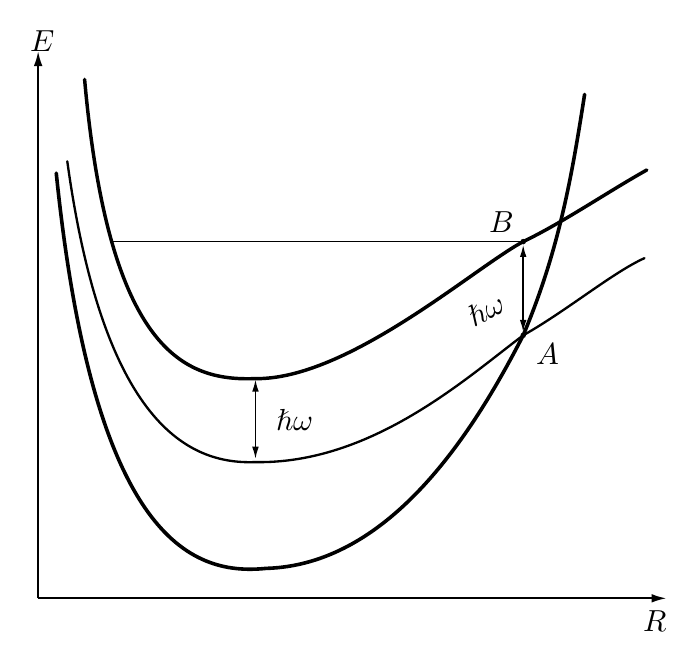
\begin{tikzpicture}[x=1cm,y=1cm]
\draw[arr] (.32,.35)--(.32,7.30);
\draw[arr] (.32,.35)--(8.30,.35);
\node[txt,anchor=south west] at (.18,7.25) {$E$};
\node[txt,anchor=north] at (8.15,.24) {$R$};
% V_0 thick lower parabola, passing through A by construction.
\draw[heavy,line width=1.30pt]
 (.55,5.75) .. controls (1.02,1.16) and (2.23,.63) .. (3.21,.73)
 .. controls (4.75,.77) and (5.81,2.38) .. (6.48,3.69)
 .. controls (6.94,4.78) and (7.10,5.73) .. (7.26,6.75);
% The thicker excited potential with visible inner minimum and right sloping branch.
\draw[heavy,line width=1.25pt]
 (.91,6.94) .. controls (1.22,3.48) and (2.18,3.11) .. (3.07,3.14)
 .. controls (4.25,3.12) and (5.86,4.55) .. (6.48,4.88)
 .. controls (6.98,5.12) and (7.55,5.51) .. (8.05,5.79);
% The displaced thin vibrational potential: lower by an indicated photon energy.
\draw[fine,line width=.84pt]
 (.69,5.90) .. controls (1.15,2.57) and (2.23,2.05) .. (3.07,2.08)
 .. controls (4.56,2.05) and (5.77,3.16) .. (6.48,3.69)
 .. controls (7.03,4.00) and (7.62,4.49) .. (8.02,4.67);
% Horizontal reference at the exact energy of point B.
\draw[fine] (1.26,4.88)--(6.48,4.88);
% Two vertical photon-energy arrows at identical R, with no unintended endpoint gaps.
\draw[dim] (3.08,2.12)--(3.08,3.13);
\node[txt,anchor=west,fill=white,inner sep=1pt] at (3.30,2.61) {$\hbar\omega$};
\draw[dim] (6.48,3.73)--(6.48,4.84);
\node[txt,anchor=east,fill=white,inner sep=1pt,rotate=27] at (6.25,4.14) {$\hbar\omega$};
\fill (6.48,3.69) circle (.035);\fill (6.48,4.88) circle (.035);
\node[txt,anchor=north west] at (6.60,3.64) {$A$};
\node[txt,anchor=south east] at (6.39,4.95) {$B$};
\end{tikzpicture}
\end{document}
